\documentclass[aspectratio=169]{beamer}

% because we need to claim weird things
\newtheorem{claim}{Claim}
\newtheorem{defn}{Definition}
%\newtheorem{lemma}{Lemma}
\newtheorem{thm}{Theorem}
\newtheorem{vita}{Vit\ae}
\newtheorem{qotd}{Quote of the Day}

\usepackage{algorithm}
\usepackage{algpseudocode}
\usepackage{listings}
\usepackage{color}
\usepackage{graphics}
\usepackage{ulem}
\bibliographystyle{unsrt}

% background image
\usebackgroundtemplate%
{%
    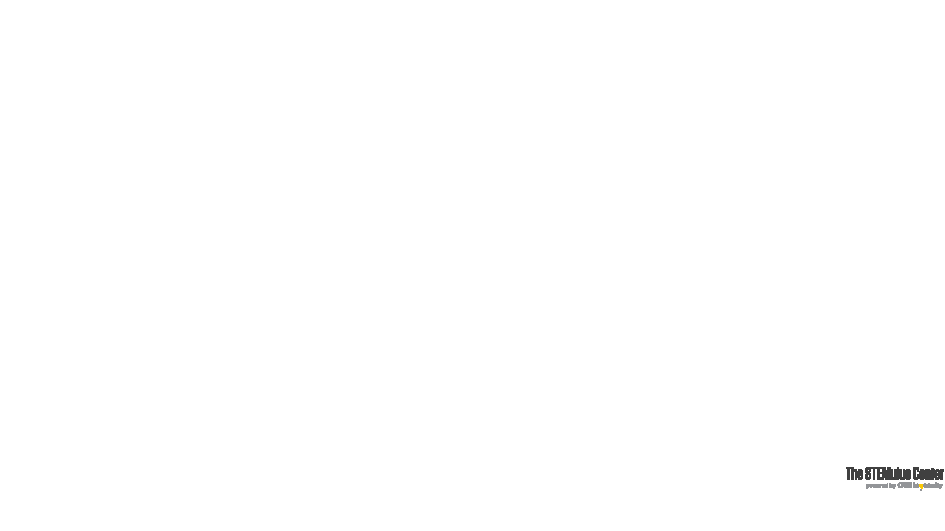
\includegraphics[width=\paperwidth,height=\paperheight]{../artifacts/stemulus.pdf}%
}
\setbeamertemplate{caption}[numbered]
\lstset{%
	breaklines=true,
	captionpos=b,
	frame=single,
	keepspaces=true,
	showstringspaces=false
}

% page numbers
\addtobeamertemplate{navigation symbols}{}{%
    \usebeamerfont{footline}%
    \usebeamercolor[fg]{footline}%
    \hspace{1em}%
    \insertframenumber/\inserttotalframenumber
}

% presentation header
\usetheme{Warsaw}
\title{Week 3: Advanced Object Oriented PHP}
\author{Dylan Lane McDonald}
\institute{CNM STEMulus Center\\Web Development with PHP}
\date{\today}

\begin{document}
\lstset{language=Java}
\begin{frame}
\titlepage
\end{frame}

\begin{frame}
\frametitle{Outline}
\tableofcontents
\end{frame}

\section{Inheritance \& Multiple Inheritance}
\subsection{Inheritance}
\begin{frame}
\frametitle{Inheritance}
\begin{defn}
\textbf{Inheritance} is when a class is based on another class. An inherited (child) class gains access to all protected and public state variables and methods. Private state variables and methods are not inherited by the child.
\end{defn}

\pause
\mbox{}\\
Inheritance is a mechanism of \textbf{code reuse} that allows a class to share code with its parent class for free. Inheritance is a \textbf{is-a} relationship. That is, child classes are considered a subset or special case of the parent class. For instance, the \textbf{HybridCar} class would be a child class of the \textbf{Car} class.

\mbox{}\\
The down side to using inheritance is that the child classes become dependent on the parent classes and are forced to contain the code propagated via inheritance.
\end{frame}

\begin{frame}[fragile]
\frametitle{Inheriting a Class}
\begin{lstlisting}[caption=Creating a Hybrid from a Car]
class HybridCar extends Car {
   protected $batteryCapacity;
   public function getBatteryCapacity() {
     return($this->batteryCapacity);
   }
}
\end{lstlisting}

The \textbf{HybridCar} class will have full access to the non-private state variables and methods in \textbf{Car}.
\end{frame}

\begin{frame}
\frametitle{\texttt{final} Keyword}
The \texttt{final} keyword prevents child classes from modifying the parent class. This has the effect of creating a read-only inheritance of \texttt{final} items. The following items can be declared \texttt{final}:
\begin{itemize}
	\item \textbf{Method}: prevents child classes from overriding methods
	\item \textbf{Class}: prevents child classes from modifying anything inheriting from the parent class
\end{itemize}
Notably absent from this list are state variables. \texttt{final} state variables can be approximated by using \href{http://php.net/manual/en/language.oop5.constants.php}{class constants}. 
\end{frame}

\subsection{Contracts \& Interfaces}
\begin{frame}
\frametitle{Contracts}
\begin{defn}
A \textbf{contract} is a collection of state variables or methods that outline the services provided by the contract and what is required to be implemented by the contract.
\end{defn}

\pause
\mbox{}\\
The term ``contract'' comes from the Java world. \cite{javapractices} The term can be likened to hiring a contractor to build another room in a house. In the house analogy, one is paying a professional to add something new to a house. In software development, a developer implements additional code with the added benefit of a service or feature provided to the program.
\end{frame}

\begin{frame}[fragile]
\frametitle{Implementing Contracts: Interfaces}
\begin{lstlisting}[caption=Creating a Hybrid Car]
interface BatteryCar {
   public function getBatteryCapacity();
}
class HybridCar implements BatteryCar {
   protected $batteryCapacity;
   public function getBatteryCapacity() {
     return($this->batteryCapacity);
   }
}
\end{lstlisting}
\end{frame}

\subsection{Traits}
\begin{frame}
\frametitle{Traits}
\begin{defn}
A \textbf{trait} is a fragment of reusable code (complete state variables and methods) that is later incorporated into a class.
\end{defn}

\pause
\mbox{}\\
Like inheritance, traits allow entire code blocks to be injected into a class. Unlike inheritance, multiple traits can be applied to a class. Inheritance only allows one parent class per child.
\end{frame}

\begin{frame}[fragile]
\frametitle{Traits}
\begin{lstlisting}[caption=Creating a Hybrid Car with a Battery Trait]
trait BatteryCarTrait {
   protected $batteryCapacity;
   public function getBatteryCapacity() {
     return($this->batteryCapacity);
   }
}
class HybridCar {
   use BatteryCarTrait;
}
\end{lstlisting}
\end{frame}

\section{Design Considerations \& the Diamond Problem}
\subsection{Diamond Problem}
\begin{frame}
\frametitle{Diamond Problem}
\begin{defn}
The \textbf{diamond problem} is a problem where methods have an ambiguous source. This is caused by using multiple inheritance and is depicted in Figure \ref{fig:diamond}.
\end{defn}
\begin{figure}
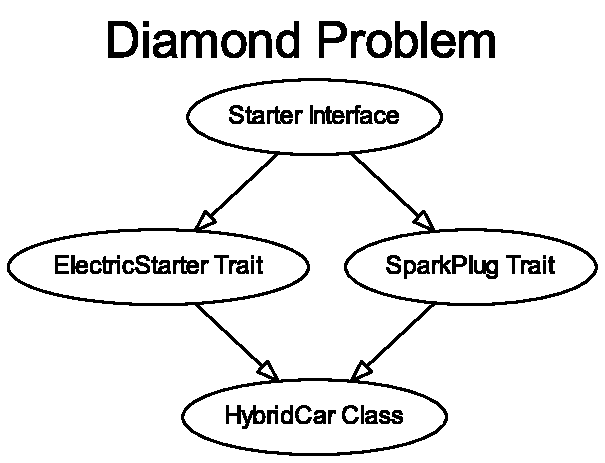
\includegraphics[scale=0.4]{../artifacts/diamond.pdf}
\caption{Diamond Problem}
\label{fig:diamond}
\end{figure}
\end{frame}

\begin{frame}[fragile]
\frametitle{Diamond Problem}
\begin{lstlisting}[caption=Diamond Problem Using Traits,label=lis:traits]
trait SparkPlug {
   public function start() {
      echo "zoom zoom";
   }
}
trait ElectricStarter {
   public function start() {
      echo "started electrically";
   }
}
\end{lstlisting}
\end{frame}

\begin{frame}[fragile]
\frametitle{Diamond Problem (Cont'd)}
\begin{lstlisting}[caption=Diamond Problem Using Traits (Cont'd),label=lis:diamond-class]
class HybridCar {
   use ElectricStarter, SparkPlug;
}
$hybrid = new HybridCar();
$hybrid->start();
\end{lstlisting}

\mbox{}\\
This illustrates the diamond problem because the \texttt{start()} method is ambiguously injected from two sources. The resolution is to either use one trait or specify where the trait comes from by writing \texttt{SparkPlug::start insteadof ElectricStarter;} as part of the \texttt{use} block.
\end{frame}

\subsection{Composing vs Inheriting}
\begin{frame}
\frametitle{Composing vs Inheriting}
The Gang of Four explicitly say, ``Favor object composition over class inheritance.'' \cite{gangoffour} Inheritance exposes the implementation of the parent class to the child classes. This is said to ``violate encapsulation'' because any change to parent classes directly affect all child classes. This is often not the desired affect. One can be more selective about which behaviors to effect by using composition instead of inheritance.

\mbox{}\\
The main advantage to composition is that it is dynamically decided at runtime, so respect for objects' interfaces is preserved, and hence, encapsulation is preserved. The end result is a system that is more robust and more flexible as business needs change.
\end{frame}

\subsection{Case Study: Strategy Design Pattern}
\begin{frame}
\frametitle{Strategy Design Pattern}
\begin{figure}
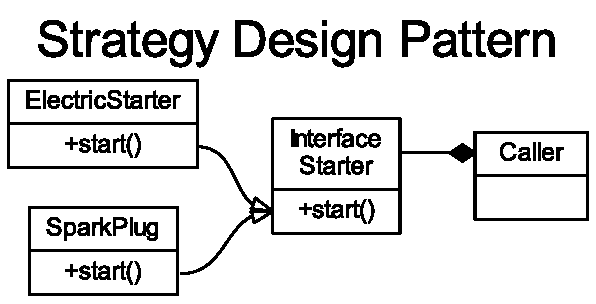
\includegraphics{../artifacts/strategy.pdf}
\caption{Strategy Design Pattern}
\label{fig:strategy}
\end{figure}
\end{frame}

\begin{frame}[fragile]
\frametitle{Strategy Design Pattern}
The traits in Listing \ref{lis:traits} can be extended to implement the \textbf{Strategy Design Pattern}. The traits can be thought of as two concrete strategies to start a Car object. Next, an interface to enforce this behavior is needed.
\begin{lstlisting}[caption=Building Out the Strategy Pattern: the Interface,label=lis:start-interface]
interface Starter {
   public function start();
}
\end{lstlisting}

\mbox{}\\
Both traits from Listing \ref{lis:traits} are candidates for this new interface because they completely implement the interface.
\end{frame}

\begin{frame}[fragile]
\frametitle{Strategy Design Pattern}
The final step is the write the class to implement the interface from Listing \ref{lis:start-interface} by simply using one of the traits from Listing \ref{lis:traits}.
\begin{lstlisting}[caption=Building Out the Strategy Pattern: the Class,label=lis:start-class]
class HybridCar implements Starter {
   use ElectricStarter;
}
\end{lstlisting}

\mbox{}\\
The extra layer introduced by the strategy design pattern allows one to interchange programmatic parts such as traits and interfaces to dynamically create classes with little work. It also adds the advantage of standardizing how all the methods behave without being concerned for what exactly the methods are doing.
\end{frame}

\begin{frame}
\frametitle{Works Cited}
\bibliography{object-oriented-advanced}
\end{frame}

\end{document}